\documentclass[border=15pt, tikz]{standalone}
\usepackage{tikz}
\usetikzlibrary{positioning, arrows.meta, calc, backgrounds}

\begin{document}

% ==============================================================================
% ESTILOS REUTILIZABLES PARA DIAGRAMAS DE SECUENCIA (DRY)
% ==============================================================================
\pagecolor{white}
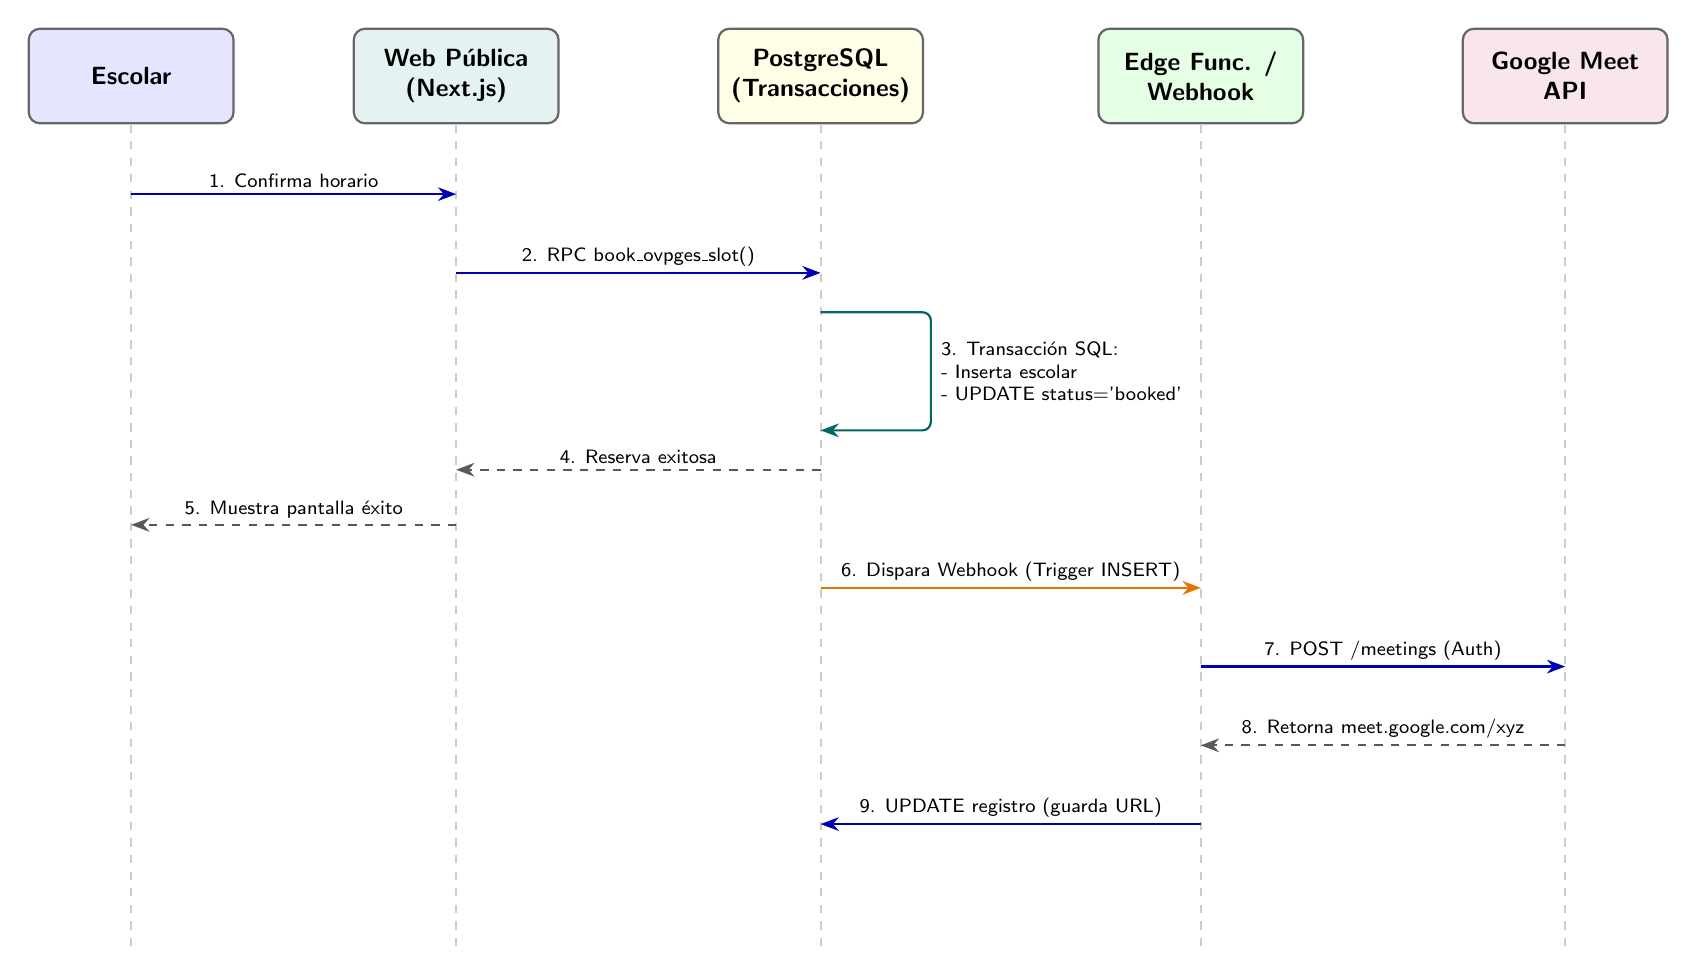
\begin{tikzpicture}[
    lifeline node/.style={
        draw=gray!80!black, fill=#1, rectangle, rounded corners,
        minimum width=2.6cm, minimum height=1.2cm, 
        font=\sffamily\small\bfseries, align=center, thick
    },
    msg/.style={->, >=Stealth, thick, draw=blue!70!black},
    ret/.style={->, >=Stealth, dashed, thick, draw=gray!70!black},
    self msg/.style={->, >=Stealth, thick, draw=teal!80!black, rounded corners=3pt},
    lbl/.style={above, font=\sffamily\scriptsize, align=center, text=black, inner sep=2pt},
    lbl right/.style={right, font=\sffamily\scriptsize, align=left, text=black}
]

% Definición de la longitud de las líneas de vida
\def\len{10.5} 

% ------------------------------------------------------------------------------
% 1. PARTICIPANTES (Posicionamiento Relativo Eje X)
% ------------------------------------------------------------------------------
\node[lifeline node=blue!10] (escolar) {Escolar};
\node[lifeline node=teal!10, right=1.5cm of escolar] (web) {Web Pública\\(Next.js)};
\node[lifeline node=yellow!10, right=2cm of web] (db) {PostgreSQL\\(Transacciones)};
\node[lifeline node=green!10, right=2.2cm of db] (edge) {Edge Func. /\\Webhook};
\node[lifeline node=purple!10, right=2cm of edge] (gmeet) {Google Meet\\API};

% ------------------------------------------------------------------------------
% 2. LÍNEAS DE VIDA (Bucle DRY)
% ------------------------------------------------------------------------------
\foreach \x in {escolar, web, db, edge, gmeet} {
    \draw[thick, gray!40, dashed] (\x.south) -- ++(0,-\len);
}

% ------------------------------------------------------------------------------
% 3. MENSAJES (Posicionamiento Relativo Eje Y mediante intersecciones |-)
% ------------------------------------------------------------------------------
% Paso 1
\draw[msg] (escolar |- 0,-1.5) -- node[lbl] {1. Confirma horario} (web |- 0,-1.5);

% Paso 2
\draw[msg] (web |- 0,-2.5) -- node[lbl] {2. RPC book\_ovpges\_slot()} (db |- 0,-2.5);

% Paso 3 (Proceso interno DB - Transacción)
\draw[self msg] (db |- 0,-3.0) -- ++(1.4,0) |- node[lbl right, near start] {3. Transacción SQL:\\- Inserta escolar\\- UPDATE status='booked'} (db |- 0,-4.5);

% Paso 4
\draw[ret] (db |- 0,-5.0) -- node[lbl] {4. Reserva exitosa} (web |- 0,-5.0);
\draw[ret] (web |- 0,-5.7) -- node[lbl] {5. Muestra pantalla éxito} (escolar |- 0,-5.7);

% Paso 6 (Webhook asíncrono)
\draw[msg, draw=orange!90!black] (db |- 0,-6.5) -- node[lbl] {6. Dispara Webhook (Trigger INSERT)} (edge |- 0,-6.5);

% Paso 7
\draw[msg] (edge |- 0,-7.5) -- node[lbl] {7. POST /meetings (Auth)} (gmeet |- 0,-7.5);

% Paso 8
\draw[ret] (gmeet |- 0,-8.5) -- node[lbl] {8. Retorna meet.google.com/xyz} (edge |- 0,-8.5);

% Paso 9
\draw[msg] (edge |- 0,-9.5) -- node[lbl] {9. UPDATE registro (guarda URL)} (db |- 0,-9.5);

\end{tikzpicture}
\end{document}
